%==============================================================================
%  Bachelor Cybersecurity -- Introduction to Machine Learning for Security
%  LaTeX Beamer deck, built in the same visual style as
%  "4_Cloud_Security_AWS_Beamer/cloud_security_master.tex".
%
%  Author: Prof. Dr.-Ing. Sebastian Schlesinger, HWR Berlin.
%  Level : BSc Business Informatics / Computer Science, 5th-6th semester.
%          Strong prior knowledge in classical cybersecurity, (almost) none in ML.
%  Build : pdflatex -> pdflatex   (run twice for TOC / frame counts)
%          or:  latexmk -pdf ml_security_intro.tex
%
%  Didactic idea (Feynman): start from the SECURITY problem, not from maths.
%  Terms are only introduced AFTER the motivation is understood. ML is framed as
%  the natural continuation of rules/signatures/heuristics -- not as a new toy.
%
%  Dramaturgy
%    0  Hook            -- why signatures/SOCs/spam no longer scale (interactive)
%    1  Classical limits-- signatures, rules, heuristics, firewalls, IDS, YARA
%    2  Security = pattern recognition (classification / anomaly detection)
%    3  ML, intuitively -- data, features, labels, function, training, inference
%    4  Learning paradigms -- supervised / unsupervised / reinforcement
%    5  ML in cybersecurity today -- EDR/XDR/SIEM/UEBA + foundation models/LLMs
%    6  What makes ML in security special -- adaptive adversary, drift, FP/FN,
%                                            explainability, adversarial ML
%    7  Practice -- red-thread board, think-pair-share, MCQ self-test, closing
%
%  Speaker notes are kept as "% Note:" comments (see instructor_guide.tex for the
%  full storyboard, live-demo scripts, think-pair-share and misconceptions).
%==============================================================================
\documentclass[aspectratio=169,10pt]{beamer}

%----------------------------------- fonts ------------------------------------
\usepackage[T1]{fontenc}
\usepackage[utf8]{inputenc}
\usepackage{lmodern}
\usepackage{microtype}

%----------------------------------- core -------------------------------------
\usepackage{xcolor}
\usepackage{booktabs}
\usepackage{array}
\usepackage{pifont}      % \ding -- check / cross / hand marks
\usepackage{listings}    % code / rule snippets
\usepackage{tikz}
\usetikzlibrary{arrows.meta,positioning,fit,backgrounds,shapes.geometric,%
                shapes.misc,calc,decorations.pathreplacing,chains}

%--------------------------------- palette ------------------------------------
\definecolor{mlink}{HTML}{172233}    % primary dark (ink)
\definecolor{mlsig}{HTML}{E8833A}    % signature accent (warm)
\definecolor{accent}{HTML}{1F6FB2}   % academic blue (structure)
\definecolor{good}{HTML}{2E7D32}     % green
\definecolor{bad}{HTML}{C62828}      % red
\definecolor{warn}{HTML}{EF6C00}     % amber
\definecolor{paleblue}{HTML}{E9F1F8}
\definecolor{lightgray}{HTML}{ECEFF1}
\definecolor{midgray}{HTML}{52606D}
\definecolor{codebg}{HTML}{F5F7FA}

%--------------------------------- theme --------------------------------------
\usetheme{default}
\setbeamertemplate{navigation symbols}{}
\setbeamersize{text margin left=0.7cm,text margin right=0.7cm}

\setbeamercolor{normal text}{fg=mlink}
\setbeamercolor{structure}{fg=accent}
\setbeamercolor{title}{fg=mlink}
\setbeamercolor{frametitle}{fg=mlink,bg=white}
\setbeamerfont{frametitle}{series=\bfseries,size=\large}
\setbeamerfont{title}{series=\bfseries,size=\LARGE}

\setbeamercolor{itemize item}{fg=mlsig}
\setbeamercolor{itemize subitem}{fg=accent}
\setbeamercolor{itemize subsubitem}{fg=midgray}
\setbeamertemplate{itemize item}{\small\raise0.2ex\hbox{\ding{110}}}
\setbeamertemplate{itemize subitem}{\footnotesize\raise0.2ex\hbox{\ding{228}}}
\setbeamertemplate{itemize subsubitem}{--}
\setbeamertemplate{enumerate items}[default]

% blocks
\setbeamertemplate{blocks}[rounded][shadow=false]
\setbeamercolor{block title}{fg=white,bg=accent}
\setbeamercolor{block body}{fg=mlink,bg=paleblue}
\setbeamercolor{block title alerted}{fg=white,bg=bad}
\setbeamercolor{block body alerted}{fg=mlink,bg=bad!8}
\setbeamercolor{block title example}{fg=white,bg=good}
\setbeamercolor{block body example}{fg=mlink,bg=good!8}

% frame title with accent rule underneath
\setbeamertemplate{frametitle}{%
  \vspace*{0.55em}%
  \begin{beamercolorbox}[wd=\paperwidth,leftskip=0.7cm,rightskip=0.7cm]{frametitle}%
    \usebeamerfont{frametitle}\insertframetitle%
    \ifx\insertframesubtitle\empty\else%
      \\[-0.15em]{\small\normalfont\color{midgray}\insertframesubtitle}%
    \fi%
  \end{beamercolorbox}%
  \vspace*{0.1em}\hspace*{0.7cm}{\color{mlsig}\rule{0.945\paperwidth}{1.1pt}}%
  \vspace*{-0.2em}%
}

% footline
\setbeamercolor{foot}{fg=midgray,bg=lightgray}
\setbeamertemplate{footline}{%
  \leavevmode%
  \hbox{%
    \begin{beamercolorbox}[wd=.34\paperwidth,ht=2.6ex,dp=1.1ex,leftskip=.7cm]{foot}%
      \tiny Bachelor Cybersecurity {\color{mlsig}\textbullet} ML for Security%
    \end{beamercolorbox}%
    \begin{beamercolorbox}[wd=.50\paperwidth,ht=2.6ex,dp=1.1ex,center]{foot}%
      \tiny\insertsectionhead%
    \end{beamercolorbox}%
    \begin{beamercolorbox}[wd=.16\paperwidth,ht=2.6ex,dp=1.1ex,rightskip=.7cm]{foot}%
      \hfill\tiny\insertframenumber\,/\,\inserttotalframenumber%
    \end{beamercolorbox}%
  }\vskip0pt%
}

% section divider slide
\AtBeginSection[]{%
  \begin{frame}[plain,noframenumbering]%
    \vfill\centering
    {\color{mlsig}\rule{0.16\paperwidth}{2.2pt}}\\[0.7em]
    {\usebeamerfont{title}\color{mlink}\insertsectionhead}\\[0.5em]
    {\color{midgray}\small Introduction to Machine Learning for Security}
    \vfill
  \end{frame}%
}

%--------------------------------- listings -----------------------------------
\lstdefinestyle{rule}{%
  basicstyle=\ttfamily\scriptsize,
  showstringspaces=false,
  breaklines=true,
  backgroundcolor=\color{codebg},
  frame=leftline,
  framerule=2.2pt,
  rulecolor=\color{mlsig},
  xleftmargin=1.1em,
  aboveskip=0.5em,belowskip=0.2em,
  stringstyle=\color{good},
  commentstyle=\color{midgray}\itshape,
  keywordstyle=\color{accent}\bfseries,
  morestring=[b]",
  morecomment=[l]{\#},
  morekeywords={rule,strings,condition,meta,and,or,not,all,any,of,them,import,%
    def,for,in,if,else,return,fit,predict,import}%
}
\lstset{style=rule}

%---------------------------------- macros ------------------------------------
\newcommand{\cmark}{\textcolor{good}{\ding{51}}}
\newcommand{\xmark}{\textcolor{bad}{\ding{55}}}
\newcommand{\term}[1]{{\color{mlink}\textbf{#1}}}         % emphasised classical term
\newcommand{\mlterm}[1]{{\color{accent}\textsf{\textbf{#1}}}} % newly introduced ML term
\newcommand{\link}[1]{{\color{accent}\small#1}}

% "Bridge to classical security" callout -- the didactic backbone of the deck:
% every ML idea is tied back to a rule/signature/heuristic the students know.
\newcommand{\bridge}[1]{%
  \begin{block}{\small\ding{43}\ Bridge to classical security}\small #1\end{block}}
% interactive question to the room
\newcommand{\ask}[1]{%
  \begin{exampleblock}{\small\ding{45}\ Ask the room}\small #1\end{exampleblock}}
% common misconception
\newcommand{\myth}[1]{%
  \begin{alertblock}{\small\ding{55}\ Common misconception}\small #1\end{alertblock}}

% TikZ reusable styles
\tikzset{
  box/.style   ={rounded corners=2pt,draw=accent,line width=0.8pt,fill=paleblue,
                 inner sep=4pt,align=center,font=\scriptsize},
  darkbox/.style={rounded corners=2pt,draw=mlink,line width=0.8pt,fill=mlink!8,
                 inner sep=4pt,align=center,font=\scriptsize},
  hot/.style   ={rounded corners=2pt,draw=bad,line width=0.9pt,fill=bad!10,
                 inner sep=4pt,align=center,font=\scriptsize},
  ok/.style    ={rounded corners=2pt,draw=good,line width=0.9pt,fill=good!10,
                 inner sep=4pt,align=center,font=\scriptsize},
  sig/.style   ={rounded corners=2pt,draw=mlsig,line width=0.9pt,fill=mlsig!12,
                 inner sep=4pt,align=center,font=\scriptsize},
  zone/.style  ={rounded corners=4pt,draw=midgray,dashed,line width=0.7pt,
                 inner sep=8pt},
  flow/.style  ={-{Stealth[length=2.2mm]},line width=0.8pt,draw=mlink},
  attack/.style={-{Stealth[length=2.2mm]},line width=0.9pt,draw=bad,dashed}
}

%---------------------------------- meta --------------------------------------
\title{Introduction to Machine Learning for Security}
\subtitle{Why security outgrew its rules --- and how machines started to learn them}
\author{Prof.\ Dr.-Ing.\ Sebastian Schlesinger}
\institute{HWR Berlin}
\date{}

%==============================================================================
\begin{document}
%==============================================================================

% Note: 90 min single lecture. Audience already knows classical security cold
% (IDS, firewalls, YARA, crypto, cloud) but has NO systematic ML background.
% Goal of the hour: the room should end up saying "now I understand WHY ML became
% necessary in security". Do NOT open with maths, datasets or algorithms.

{\setbeamertemplate{footline}{}
\begin{frame}[plain,noframenumbering]
  \vspace*{0.4cm}
  \begin{tikzpicture}[remember picture,overlay]
    \fill[mlink] (current page.north west) rectangle ([yshift=-2.0cm]current page.north east);
    \node[anchor=west,text=white] at ([xshift=0.9cm,yshift=-1.0cm]current page.north west)
      {\Large\bfseries Cybersecurity Master};
    \fill[mlsig] ([yshift=-2.0cm]current page.north west) rectangle ([yshift=-2.12cm]current page.north east);
  \end{tikzpicture}
  \vspace*{2.6cm}

  {\usebeamerfont{title}\color{mlink}\inserttitle}\\[0.3em]
  {\large\color{midgray}\insertsubtitle}\\[1.4em]
  {\color{mlink}\insertauthor}\\[0.2em]
  {\small\color{midgray}\insertinstitute}
\end{frame}}

%------------------------------------------------------------------------------
% \begin{frame}{Agenda --- we follow a story, not a syllabus}
%   \footnotesize
%   \begin{columns}[T]
%     \begin{column}{0.5\textwidth}
%       \textbf{\color{accent}Part I --- The problem}
%       \begin{enumerate}\setlength\itemsep{1pt}
%         \item The hook: security that no longer scales
%         \item Why classical methods hit a wall
%         \item Security \emph{is} pattern recognition
%       \end{enumerate}
%       \vspace{0.6em}
%       \textbf{\color{accent}Part II --- The idea}
%       \begin{enumerate}\setlength\itemsep{1pt}\setcounter{enumi}{3}
%         \item Machine learning, intuitively
%         \item The three learning paradigms
%       \end{enumerate}
%     \end{column}
%     \begin{column}{0.5\textwidth}
%       \textbf{\color{accent}Part III --- The reality}
%       \begin{enumerate}\setlength\itemsep{1pt}\setcounter{enumi}{5}
%         \item Where ML lives in security today
%         \item What makes ML in security \emph{special}
%       \end{enumerate}
%       \vspace{0.6em}
%       \textbf{\color{accent}Part IV --- Practice}
%       \begin{itemize}\setlength\itemsep{1pt}
%         \item The red-thread board
%         \item Think--pair--share \& MCQ self-test
%         \item The one message to take home
%       \end{itemize}
%     \end{column}
%   \end{columns}
%   \vfill
%   {\footnotesize\color{midgray}No maths prerequisites. Every new term is introduced
%   \emph{after} the problem that needs it.}
% \end{frame}

% \begin{frame}{Learning goals for today}
%   % Note: read these out; return to them on the summary slide.
%   \begin{itemize}
%     \item Explain \term{why} rule-, signature- and heuristic-based security is
%           hitting fundamental limits --- in your own words, from your own modules.
%     \item Reframe classic security tasks (malware, spam, IDS, fraud, User Entity Behaviour Analysis (UEBA)) as
%           \mlterm{classification} or \mlterm{anomaly detection} problems.
%     \item Describe --- without maths --- what \mlterm{data}, \mlterm{features},
%           \mlterm{labels}, \mlterm{training}, \mlterm{inference} and
%           \mlterm{generalisation} mean.
%     \item Distinguish \mlterm{supervised}, \mlterm{unsupervised} and
%           \mlterm{reinforcement} learning by their security use cases.
%     \item Name where ML runs in modern defence (EDR/XDR/SIEM/UEBA) and why the
%           \term{adaptive adversary} makes security ML unlike any other ML.
%   \end{itemize}
%   \vfill
%   {\footnotesize\color{midgray}Today is the ``why''. The rest of the series is
%   the ``how''.}
% \end{frame}

%##############################################################################
%  PART I -- THE PROBLEM
%##############################################################################

%==============================================================================
\section{The hook: security that no longer scales}
%==============================================================================

\begin{frame}{You are on the SOC night shift}
  % Note: OPEN HERE. Do not mention ML for the first ~12 minutes. Let them feel
  % the problem. Ask before revealing the number.
  \begin{columns}[T]
    \begin{column}{0.55\textwidth}
      \begin{itemize}
        \item It is 03:00. You are the only analyst on shift.
        \item Your \term{Security Information and Event Management (SIEM)} shows the events collected in the last 24\,h.
        \item Each one \emph{could} be the first step of a breach --- or nothing.
      \end{itemize}
      \vspace{0.4em}
      \ask{How many security events does a mid-size enterprise SOC ingest per day?
      Shout a number.\\[0.2em]
      \footnotesize (Order of magnitude: \textbf{$10^9$--$10^{10}$} events/day.
      One human reviews maybe a few hundred.)}
    \end{column}
    \begin{column}{0.45\textwidth}
      \centering
      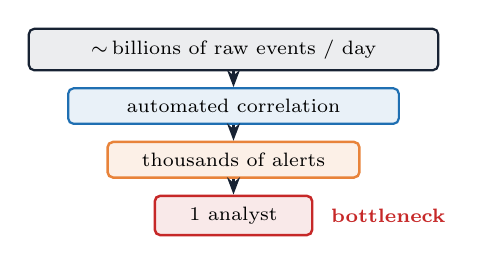
\begin{tikzpicture}[node distance=2mm,every node/.style={font=\scriptsize}]
        \node[darkbox,minimum width=5.2cm] (raw) {$\sim$\,billions of raw events / day};
        \node[box,minimum width=4.2cm,below=of raw] (corr) {automated correlation};
        \node[sig,minimum width=3.2cm,below=of corr] (alert) {thousands of alerts};
        \node[hot,minimum width=2.0cm,below=of alert] (human) {1 analyst};
        \draw[flow] (raw) -- (corr);
        \draw[flow] (corr) -- (alert);
        \draw[flow] (alert) -- (human);
        \node[right=1mm of human,text=bad,font=\scriptsize\bfseries] {bottleneck};
      \end{tikzpicture}
      \par\vspace{0.3em}
      {\footnotesize\color{midgray}The funnel is real. The bottleneck is human.}
    \end{column}
  \end{columns}
\end{frame}

\begin{frame}{The number that breaks the old model}
  % Note: this is the emotional core of the hook. Let the malware number land.
  \begin{columns}[T]
    \begin{column}{0.52\textwidth}
      \begin{itemize}
        \item \term{AV-TEST} registers roughly \textbf{450{,}000 new malware
              samples \emph{every day}} --- $>$\,100 per second.
        \item Classic antivirus works by \term{signatures}: a fingerprint per
              known bad file.
        \item So the honest question is very simple\ldots
      \end{itemize}
      \ask{\textbf{Can we write --- and ship --- one hand-crafted signature for
      every new sample, forever?}\\[0.2em]
      %\footnotesize Let them answer. The answer is obviously ``no''. \emph{That}
      %``no'' is the reason this lecture exists.
      }
    \end{column}
    \begin{column}{0.48\textwidth}
      \centering
      % schematic: demand grows, hand-written supply is flat
      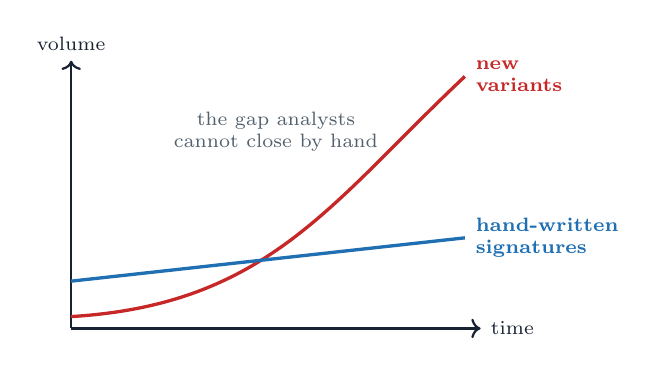
\begin{tikzpicture}[font=\scriptsize]
        \draw[->,thick,mlink] (0,0) -- (5.2,0) node[right]{time};
        \draw[->,thick,mlink] (0,0) -- (0,3.4) node[above,align=center]{volume};
        \draw[very thick,bad] (0,0.15) .. controls (2.5,0.3) and (3.3,1.6) .. (5.0,3.2)
          node[right,text=bad,align=left,font=\scriptsize\bfseries]{new\\variants};
        \draw[very thick,accent] (0,0.6) -- (5.0,1.15)
          node[right,text=accent,align=left,font=\scriptsize\bfseries]{hand-written\\signatures};
        \node[text=midgray,align=center,font=\scriptsize] at (2.6,2.5)
          {the gap analysts\\cannot close by hand};
      \end{tikzpicture}
    \end{column}
  \end{columns}
\end{frame}

\begin{frame}{Three everyday problems, one shared shape}
  % Note: quick round. Get them to spot that all three are "sort into good/bad
  % at a scale and speed no human or fixed rule can match". Do NOT name ML yet.
  \small
  \renewcommand{\arraystretch}{1.35}
  \begin{tabular}{>{\raggedright\arraybackslash}p{2.7cm} >{\raggedright\arraybackslash}p{5.6cm} >{\raggedright\arraybackslash}p{3.4cm}}
    \toprule
    \textbf{Problem} & \textbf{Why a fixed rule struggles} & \textbf{What we actually want}\\
    \midrule
    Spam in your inbox & Wording changes hourly; ``free'' vs ``fr\_ee'' vs an image & keep good mail, drop bad\\
    Malware on an endpoint & 450k new samples/day, packers, polymorphism & allow benign, block malicious\\
    Zero-day intrusion & By definition \emph{no} signature exists yet & flag ``this is not normal''\\
    \bottomrule
  \end{tabular}
  \vfill
  \begin{block}{\small The shape of all three}
    \small A stream of \term{objects} arrives; for each we must make a fast
    \term{good / bad} (or \term{normal / weird}) \term{decision}, at a volume and
    variability no analyst and no static list can keep up with.
  \end{block}
  % Note: hold this thought. We will call this "shape" pattern recognition in 15 min.
\end{frame}

%==============================================================================
\section{Why classical methods hit a wall}
%==============================================================================

\begin{frame}{The classical toolbox --- which you already master}
  % Note: this is a RESPECT slide. These methods are not obsolete; they are the
  % foundation. We are extending them, not replacing them. Ask students to fill in.
  \small
  \renewcommand{\arraystretch}{1.3}
  \begin{tabular}{>{\raggedright\arraybackslash}p{3.0cm} >{\raggedright\arraybackslash}p{5.3cm} >{\raggedright\arraybackslash}p{3.4cm}}
    \toprule
    \textbf{Method} & \textbf{How it decides} & \textbf{You met it in}\\
    \midrule
   % Signatures (AV, IDS)   & exact/known-bad fingerprint match      & Malware, Network Sec.\\
    Rule-based systems      & hand-written \texttt{if\dots then} logic & Firewalls, SIEM correlation\\
    Heuristics              & expert ``rules of thumb'', scoring     & Spam filters, EDR\\
    Firewalls / ACLs        & allow/deny by port, IP, protocol       & Network Security\\
    IDS/IPS (signature)     & match traffic to known attack patterns & Intrusion Detection\\
    %YARA rules              & byte/string patterns in files          & Malware analysis\\
    \bottomrule
  \end{tabular}
  \vfill
  {\footnotesize\color{midgray}Common thread: a \emph{human} encodes ``what bad
  looks like'' \emph{in advance}, explicitly.}
\end{frame}

\begin{frame}[fragile]{A rule, made concrete --- a YARA signature}
  % Note: show something they recognise. Then ask what an attacker changes to slip past.
  \begin{columns}[T]
    \begin{column}{0.56\textwidth}
      \begin{lstlisting}[language=]
rule Suspicious_Downloader {
  meta:
    author = "SOC team"
  strings:
    $a = "http://evil.example/payload"
    $b = { 6A 40 68 00 30 00 00 }   // opcodes
    $c = "InternetOpenA"
  condition:
    2 of ($a, $b, $c)
}
      \end{lstlisting}

      \begin{block}{What is YARA?}
        YARA is a tool designed to identify and classify malware. It uses a simple syntax to define rules that can be used to detect specific patterns in files or memory.
      \end{block}
    \end{column}
    \begin{column}{0.44\textwidth}
      \begin{itemize}\small
        \item Precise, fast, \term{explainable}: you know \emph{exactly} why it
              fired.
        \item Zero false positives --- \emph{on what it was written for}.
      \end{itemize}
      \ask{You are the attacker. Name \emph{one} trivial change that defeats this
      rule.\\[0.2em]
     % \footnotesize (rename the URL, re-encrypt the payload, XOR the strings,
      %re-order opcodes\ldots each breaks an exact match.)
      }
    \end{column}
  \end{columns}
  % Note: the punchline -- an exact rule is brittle exactly where the adversary is free.
\end{frame}

\begin{frame}{Where the wall is --- five structural limits}
  % Note: co-develop this list WITH the room; they will produce most of it.
  \begin{columns}[T]
    \begin{column}{0.6\textwidth}
      \begin{enumerate}\setlength\itemsep{3pt}
        \item \term{Scale.} One rule per threat $\times$ millions of new threats
              $=$ a list nobody can maintain.
        \item \term{Novelty.} A \term{zero-day} has, by definition, no signature.
              Rules only catch the past.
        \item \term{Evasion.} Rules are public logic; \term{polymorphism} and
              obfuscation are cheap for the attacker.
        \item \term{Combinatorics.} ``Bad'' is a fuzzy blend of hundreds of weak
              hints --- too many to enumerate by hand.
        \item \term{Maintenance.} Every rule is a false-positive risk and a
              forever cost. Rulesets rot.
      \end{enumerate}
    \end{column}
    \begin{column}{0.4\textwidth}
      \centering
      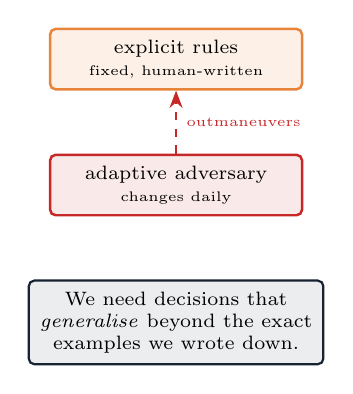
\begin{tikzpicture}[font=\scriptsize,node distance=3mm]
        \node[sig,minimum width=3.2cm] (r) {explicit rules\\\tiny fixed, human-written};
        \node[hot,below=8mm of r,minimum width=3.2cm] (a) {adaptive adversary\\\tiny changes daily};
        \draw[attack] (a) -- node[right,text=bad,font=\tiny]{outmaneuvers} (r);
        \node[darkbox,below=8mm of a,minimum width=3.6cm] (need)
          {We need decisions that\\\emph{generalise} beyond the exact\\examples we wrote down.};
      \end{tikzpicture}
    \end{column}
  \end{columns}
  \myth{``Then just write better/more rules.'' --- More rules means more false
  positives, more maintenance, and still zero coverage of the genuinely new.}
\end{frame}

%==============================================================================
\section{Security is pattern recognition}
%==============================================================================

\begin{frame}{The re-frame: it was a classification problem all along}
  % Note: THE PIVOT of the lecture. Slow down. This is the "aha".
  \centering
  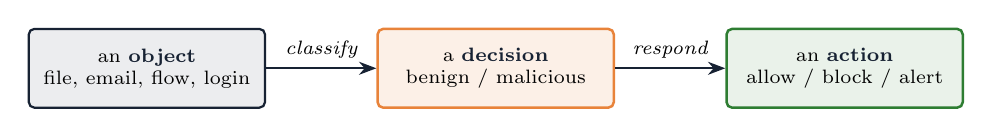
\begin{tikzpicture}[font=\small,node distance=6mm]
    \node[darkbox,minimum width=3.0cm,minimum height=1.0cm] (obj) {an \term{object}\\\scriptsize file, email, flow, login};
    \node[sig,right=14mm of obj,minimum width=3.0cm,minimum height=1.0cm] (dec) {a \term{decision}\\\scriptsize benign / malicious};
    \node[ok,right=14mm of dec,minimum width=3.0cm,minimum height=1.0cm] (act) {an \term{action}\\\scriptsize allow / block / alert};
    \draw[flow] (obj) -- node[above,font=\scriptsize\itshape]{classify} (dec);
    \draw[flow] (dec) -- node[above,font=\scriptsize\itshape]{respond} (act);
  \end{tikzpicture}
  \vfill
  \begin{columns}[T]
    \begin{column}{0.5\textwidth}
      \begin{block}{\small Classification}
        \small ``Which known \emph{category} does this object belong to?''
        --- benign vs malicious, spam vs ham, this-of-5-malware-families.
      \end{block}
    \end{column}
    \begin{column}{0.5\textwidth}
      \begin{block}{\small Anomaly detection}
        \small ``Does this object \emph{deviate} from normal?'' --- for when we
        cannot enumerate ``bad'', only ``usual'' (great for zero-days).
      \end{block}
    \end{column}
  \end{columns}
  \vfill
  {\footnotesize\color{midgray}Signatures were always doing classification ---
  just with a rulebook a human had to write by hand.}
\end{frame}

\begin{frame}{Your whole curriculum, viewed as pattern recognition}
  % Note: go fast, one line each. For each: object / decision / why rules get hard.
  \scriptsize
  \renewcommand{\arraystretch}{1.25}
  \begin{tabular}{>{\raggedright\arraybackslash}p{2.5cm} >{\raggedright\arraybackslash}p{3.2cm} >{\raggedright\arraybackslash}p{3.0cm} >{\raggedright\arraybackslash}p{4.0cm}}
    \toprule
    \textbf{Task} & \textbf{Object} & \textbf{Decision} & \textbf{Why explicit rules get hard}\\
    \midrule
    Malware detection   & a file / process    & benign / malicious      & packers, polymorphism, 450k/day\\
    Spam detection      & an email            & spam / ham              & wording mutates hourly\\
    Phishing detection  & a URL / page        & phishing / legit        & look-alikes, new domains constantly\\
    Intrusion detection & a network flow      & normal / attack         & encrypted, blends into traffic\\
    UEBA                & a user's behaviour  & typical / suspicious    & ``normal'' differs per person\\
    Fraud detection     & a transaction       & legit / fraud           & fraud mimics real behaviour\\
    Cloud anomalies     & API call / config   & expected / risky        & millions of calls, changing baselines\\
    DNS tunnelling      & DNS queries         & benign / exfiltration   & looks like ordinary DNS\\
    Bot detection       & a session / client  & human / bot             & bots imitate humans\\
    \bottomrule
  \end{tabular}
  \vfill
  {\footnotesize\color{midgray}Same shape every row: \emph{object $\to$ decision},
  where ``bad'' is too varied, too new, or too subtle to fully write down.}
\end{frame}

\begin{frame}{Two worked examples --- object, decision, why rules fail}
  \begin{columns}[T]
    \begin{column}{0.5\textwidth}
      \begin{exampleblock}{\small DNS tunnelling}
        \small
        \textbf{Object:} the stream of DNS queries from a host.\\
        \textbf{Decision:} ordinary name lookups vs data smuggled out.\\
        \textbf{Why rules fail:} a single query looks fine; the \emph{pattern}
        (length, entropy, rate, rare subdomains) is the tell --- and thresholds
        that catch it also flag legit CDNs.
      \end{exampleblock}
    \end{column}
    \begin{column}{0.5\textwidth}
      \begin{exampleblock}{\small UEBA (insider / account takeover)}
        \small
        \textbf{Object:} what one user does today.\\
        \textbf{Decision:} their usual behaviour vs someone else on their account.\\
        \textbf{Why rules fail:} there is no global ``normal'' --- a 2\,a.m.\
        login is fine for an admin, alarming for HR. Normal is \emph{per person}.
      \end{exampleblock}
    \end{column}
  \end{columns}
  \vfill
  \begin{block}{\small The uncomfortable conclusion}
    \small For these, nobody can hand-write the rule --- but we \emph{do} have
    piles of \term{examples} of normal and abnormal. \emph{What if the machine
    could read the rule off the examples itself?}
  \end{block}
  % Note: this sentence is the hand-off into Part II. Pause here.
\end{frame}

%##############################################################################
%  PART II -- THE IDEA
%##############################################################################

%==============================================================================
\section{Machine learning, intuitively}
%==============================================================================

\begin{frame}{The one idea behind all of machine learning}
  % Note: FIRST time we say "machine learning" with intent. Keep it plain.
  \begin{columns}[T]
    \begin{column}{0.5\textwidth}
      \centering
      \textbf{\color{bad}Classical}\\[0.3em]
      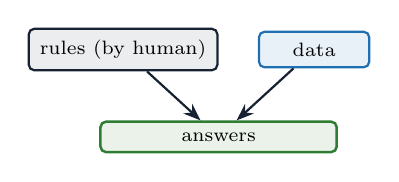
\begin{tikzpicture}[font=\scriptsize,node distance=3mm]
        \node[darkbox,minimum width=2.2cm] (rules) {rules (by human)};
        \node[box,right=5mm of rules,minimum width=1.4cm] (data1) {data};
        \node[ok,below=9mm of $(rules)!0.5!(data1)$,minimum width=3.0cm] (ans1) {answers};
        \draw[flow] (rules) -- (ans1);
        \draw[flow] (data1) -- (ans1);
      \end{tikzpicture}
      \par\vspace{0.3em}{\scriptsize humans write rules $\to$ program applies them}
    \end{column}
    \begin{column}{0.5\textwidth}
      \centering
      \textbf{\color{good}Machine learning}\\[0.3em]
      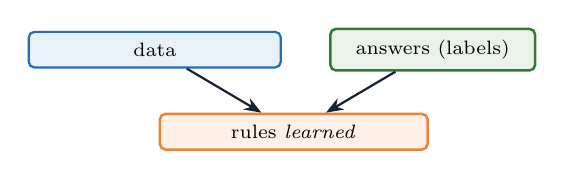
\begin{tikzpicture}[font=\scriptsize,node distance=3mm]
        \node[box,minimum width=3.2cm] (data2) {data};
        \node[ok,right=6mm of data2,minimum width=2.6cm] (ans2) {answers (labels)};
        \node[sig,below=8mm of $(data2)!0.5!(ans2)$,minimum width=3.4cm] (rules2) {rules \emph{learned}};
        \draw[flow] (data2) -- (rules2);
        \draw[flow] (ans2) -- (rules2);
      \end{tikzpicture}
      \par\vspace{0.3em}{\scriptsize show examples $+$ answers $\to$ machine infers the rule}
    \end{column}
  \end{columns}
  \vfill
  \begin{block}{\small In one line}
    \small \mlterm{Machine learning} $=$ instead of \emph{writing} the decision
    rule, we \emph{learn} it from examples --- so it can generalise to objects we
    never explicitly listed.
  \end{block}
  \bridge{A signature is a rule you wrote. A trained model is a rule the data
  wrote. Same job (classify), different author.}
\end{frame}

\begin{frame}{Data, features, labels --- said without maths}
  % Note: build the spam feature vector live on the whiteboard (see instructor guide).
  \begin{columns}[T]
    \begin{column}{0.56\textwidth}
      \begin{itemize}
        \item \mlterm{Data:} the raw objects --- e.g.\ 100k emails you kept.
        \item \mlterm{Features:} the measurable clues per object. For an email:
              \emph{\#links, \% capitals, has ``invoice'', sender age, attachment
              type\ldots} --- turning an object into numbers.
        \item \mlterm{Label:} the known answer for training examples ---
              \texttt{spam} or \texttt{ham}.
        \item Feature engineering \emph{is} the security expertise: you already
              know which clues matter.
      \end{itemize}
      \bridge{``Features'' are exactly the \emph{indicators} you put in a YARA or
      SIEM rule --- but now they are \emph{inputs to be weighed}, not a hard
      threshold you fix by hand.}
    \end{column}
    \begin{column}{0.44\textwidth}
      \centering
      \scriptsize
      \renewcommand{\arraystretch}{1.2}
      \begin{tabular}{lccc c}
        \toprule
        email & \#links & \%CAPS & ``invoice'' & label\\
        \midrule
        $e_1$ & 9  & 40 & yes & \textcolor{bad}{spam}\\
        $e_2$ & 1  & 5  & no  & \textcolor{good}{ham}\\
        $e_3$ & 12 & 60 & yes & \textcolor{bad}{spam}\\
        $e_4$ & 0  & 8  & no  & \textcolor{good}{ham}\\
        $e_5$ & 7  & 33 & yes & \textcolor{bad}{spam}\\
        \bottomrule
      \end{tabular}
      \par\vspace{0.5em}
      {\color{midgray}Each row = one object as a \emph{feature vector} $+$ its label.}
    \end{column}
  \end{columns}
\end{frame}

\begin{frame}{Learning a function = drawing the boundary}
  % Note: this picture is the whole intuition of supervised learning. Draw it live too.
  \begin{columns}[T]
    \begin{column}{0.5\textwidth}
      \centering
      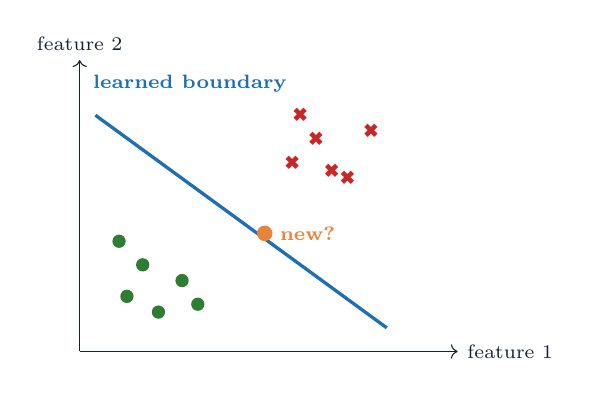
\begin{tikzpicture}[font=\scriptsize]
        \draw[->,mlink] (0,0) -- (4.8,0) node[right]{feature 1};
        \draw[->,mlink] (0,0) -- (0,3.7) node[above]{feature 2};
        % ham (good) lower-left
        \foreach \p in {(0.6,0.7),(1.0,0.5),(0.8,1.1),(1.3,0.9),(0.5,1.4),(1.5,0.6)}
          \fill[good] \p circle (2.4pt);
        % spam (bad) upper-right
        \foreach \p in {(3.0,2.7),(3.4,2.2),(2.8,3.0),(3.7,2.8),(3.2,2.3),(2.7,2.4)}
          \node[bad] at \p {\ding{54}};
        % boundary (label moved to the clear top-left, above the point clouds)
        \draw[very thick,accent] (0.2,3.0) -- (3.9,0.3);
        \node[text=accent,font=\scriptsize\bfseries] at (1.4,3.4) {learned boundary};
        % a new point sitting on the boundary; label to its right in clear space
        \fill[mlsig] (2.35,1.5) circle (2.8pt);
        \node[mlsig,font=\scriptsize\bfseries,right=2pt] at (2.35,1.5) {new?};
      \end{tikzpicture}
    \end{column}
    \begin{column}{0.5\textwidth}
      \begin{itemize}\small
        \item \mlterm{Training:} nudge the boundary until it separates the
              labelled examples well.
        \item \mlterm{Inference:} a new object arrives $\to$ which side of the
              boundary is it on? $\to$ that is the prediction.
        \item \mlterm{Generalisation:} the boundary must work on \emph{unseen}
              objects (the orange point), not just memorise the training set.
      \end{itemize}
      \myth{``The model memorises all the malware.'' It does not store the
      samples --- it learns a \emph{boundary}. That is why it can flag a variant
      it has never seen.}
    \end{column}
  \end{columns}
  % Note: name overfitting only lightly -- a boundary that wiggles around every dot fails on new data.
\end{frame}

\begin{frame}{Training vs.\ inference --- the two clocks of every ML system}
  \centering
  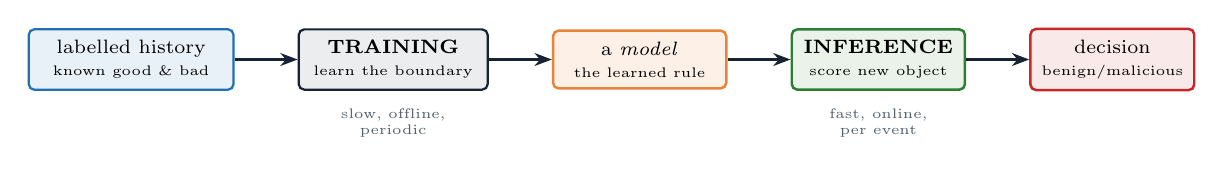
\begin{tikzpicture}[font=\scriptsize,node distance=8mm]
    \node[box,minimum width=2.6cm] (hist) {labelled history\\\tiny known good \& bad};
    \node[darkbox,right=of hist,minimum width=2.4cm] (train) {\textbf{TRAINING}\\\tiny learn the boundary};
    \node[sig,right=of train,minimum width=2.2cm] (model) {a \emph{model}\\\tiny the learned rule};
    \node[ok,right=of model,minimum width=2.2cm] (infer) {\textbf{INFERENCE}\\\tiny score new object};
    \node[hot,right=of infer,minimum width=2.0cm] (out) {decision\\\tiny benign/malicious};
    \draw[flow] (hist) -- (train);
    \draw[flow] (train) -- (model);
    \draw[flow] (model) -- (infer);
    \draw[flow] (infer) -- (out);
    \node[below=1mm of train,text=midgray,font=\tiny,align=center] {slow, offline,\\periodic};
    \node[below=1mm of infer,text=midgray,font=\tiny,align=center] {fast, online,\\per event};
  \end{tikzpicture}
  \vfill
  \begin{columns}[T]
    \begin{column}{0.5\textwidth}
      \bridge{Inference is the run-time check --- the moral equivalent of the IDS
      matching a packet. It just uses a \emph{learned} rule instead of a written
      one.}
    \end{column}
    \begin{column}{0.5\textwidth}
      \myth{``The AI keeps learning live from every attack.'' Usually not:
      most systems \emph{train periodically} and only \emph{infer} in real time.
      Continuous learning is a deliberate (and risky) design choice.}
    \end{column}
  \end{columns}
\end{frame}

%==============================================================================
\section{The three learning paradigms}
%==============================================================================

\begin{frame}{Three ways a machine can learn --- each maps to security}
  \centering
  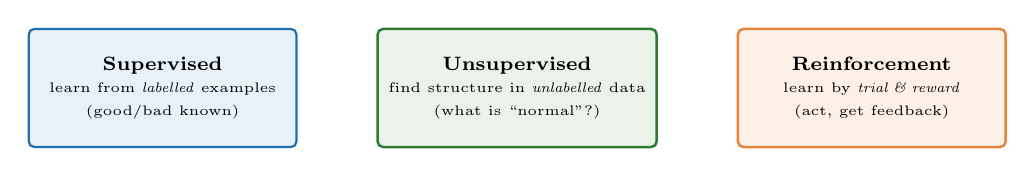
\begin{tikzpicture}[font=\scriptsize,node distance=10mm]
    \node[box,minimum width=3.4cm,minimum height=1.5cm] (sup)
      {\textbf{Supervised}\\\tiny learn from \emph{labelled} examples\\\tiny (good/bad known)};
    \node[ok,right=of sup,minimum width=3.4cm,minimum height=1.5cm] (uns)
      {\textbf{Unsupervised}\\\tiny find structure in \emph{unlabelled} data\\\tiny (what is ``normal''?)};
    \node[sig,right=of uns,minimum width=3.4cm,minimum height=1.5cm] (rl)
      {\textbf{Reinforcement}\\\tiny learn by \emph{trial \& reward}\\\tiny (act, get feedback)};
  \end{tikzpicture}
  \vfill
  \small
  \renewcommand{\arraystretch}{1.25}
  \begin{tabular}{>{\raggedright\arraybackslash}p{2.6cm} >{\raggedright\arraybackslash}p{4.6cm} >{\raggedright\arraybackslash}p{5.0cm}}
    \toprule
    \textbf{Paradigm} & \textbf{You give it\ldots} & \textbf{Security example}\\
    \midrule
    Supervised    & objects \emph{plus} the right answers & spam/malware/phishing classifiers\\
    Unsupervised  & objects only, no answers              & UEBA, network anomaly detection\\
    Reinforcement & an environment \& a reward signal     & auto-response, adaptive honeypots, fuzzing\\
    \bottomrule
  \end{tabular}
\end{frame}

\begin{frame}{Supervised learning --- the workhorse of detection}
  \begin{columns}[T]
    \begin{column}{0.58\textwidth}
      \begin{itemize}
        \item You have \term{labels}: a corpus of known malware \emph{and} known
              benign files.
        \item The model learns the boundary between the two classes.
        \item New file $\to$ ``\textbf{92\% malicious}'' $\to$ block.
        \item Most commercial malware/phishing/spam detection is here.
      \end{itemize}
      \bridge{This is your AV/IDS \emph{signature}, generalised: instead of
      matching one known-bad, it recognises the \emph{family resemblance} to
      thousands of known-bad --- so a fresh variant still trips it.}
    \end{column}
    \begin{column}{0.42\textwidth}
      \begin{block}{\small The catch (Part III)}
        \small Supervised learning is only as good as its labels. In security,
        labels are \emph{scarce, expensive, and often wrong} --- attackers hide,
        so ``benign'' may just be ``not caught yet''.
      \end{block}
      \myth{``More data always means a better model.'' Mislabelled or biased data
      makes it confidently wrong.}
    \end{column}
  \end{columns}
\end{frame}

\begin{frame}{Unsupervised learning --- when you cannot label ``bad''}
  \begin{columns}[T]
    \begin{column}{0.5\textwidth}
      \begin{itemize}
        \item No labels: you only have \emph{normal} operations logged.
        \item The model learns a \term{baseline} of ``usual'', then flags what
              \emph{deviates} --- \mlterm{anomaly detection}.
        \item Perfect for \term{zero-days} and \term{insiders}: you need not have
              seen the attack before, only ``this isn't normal''.
        \item Also \mlterm{clustering}: group similar malware into families
              automatically.
      \end{itemize}
      \bridge{This is UEBA and network baselining --- the ML version of ``I know
      what my network usually looks like, and \emph{that} is new''.}
    \end{column}
    \begin{column}{0.5\textwidth}
      \centering
      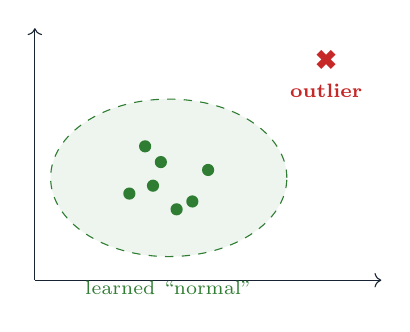
\begin{tikzpicture}[font=\scriptsize]
        \draw[->,mlink] (0,0) -- (4.4,0);
        \draw[->,mlink] (0,0) -- (0,3.2);
        \node[draw=good,dashed,ellipse,minimum width=3.0cm,minimum height=2.0cm,
              fill=good!8] at (1.7,1.3) {};
        \foreach \p in {(1.2,1.1),(1.6,1.5),(2.0,1.0),(1.4,1.7),(2.2,1.4),(1.8,0.9),(1.5,1.2)}
          \fill[good] \p circle (2.2pt);
        \node[bad,font=\bfseries] at (3.7,2.8) {\ding{54}};
        \node[bad,font=\scriptsize\bfseries] at (3.7,2.4) {outlier};
        \node[good,font=\scriptsize] at (1.7,-0.1) {learned ``normal''};
      \end{tikzpicture}
      \par\vspace{0.3em}
      {\footnotesize\color{midgray}No labels needed --- only a notion of ``far
      from usual''.}
    \end{column}
  \end{columns}
\end{frame}

\begin{frame}{Reinforcement learning --- learning to act, not just to judge}
  \begin{columns}[T]
    \begin{column}{0.56\textwidth}
      \begin{itemize}
        \item An \term{agent} takes an \term{action}, sees the result, gets a
              \term{reward}, and adjusts --- learning a \emph{policy} by trial.
        \item Security uses (mostly emerging):
        \begin{itemize}
          \item \term{Automated response}: which containment action minimises
                damage?
          \item \term{Adaptive honeypots} that keep an attacker engaged.
          \item \term{Fuzzing / pentest agents} that learn which inputs break a
                target.
        \end{itemize}
        \item The same idea powers game-playing agents (Go, Atari).
      \end{itemize}
      \bridge{Think of a \term{SOAR} playbook that \emph{tunes itself}: it tries
      responses and keeps what worked --- instead of a fixed, human-authored
      runbook.}
    \end{column}
    \begin{column}{0.44\textwidth}
      \centering
      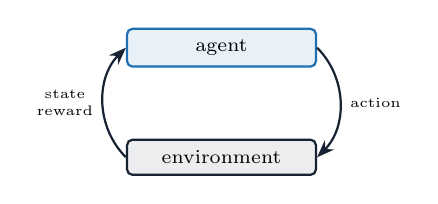
\begin{tikzpicture}[font=\scriptsize,node distance=9mm]
        \node[box,minimum width=2.4cm] (agent) {agent};
        \node[darkbox,below=of agent,minimum width=2.4cm] (env) {environment};
        \draw[flow] (agent.east) to[bend left=45] node[right,font=\tiny]{action} (env.east);
        \draw[flow] (env.west) to[bend left=45] node[left,align=center,font=\tiny]{state\\reward} (agent.west);
      \end{tikzpicture}
      \par\vspace{0.4em}
      {\footnotesize\color{midgray}Least mature in production security --- but the
      research frontier for autonomous defence \emph{and} attack.}
    \end{column}
  \end{columns}
\end{frame}

%##############################################################################
%  PART III -- THE REALITY
%##############################################################################

%==============================================================================
\section{Where ML lives in security today}
%==============================================================================

\begin{frame}{You are already surrounded by security ML}
  % Note: connect each acronym to a paradigm they now understand.
  \small
  \renewcommand{\arraystretch}{1.3}
  \begin{tabular}{>{\raggedright\arraybackslash}p{3 cm} >{\raggedright\arraybackslash}p{6.6cm} >{\raggedright\arraybackslash}p{3.0cm}}
    \toprule
    \textbf{Where} & \textbf{What the ML does} & \textbf{Mostly which paradigm}\\
    \midrule
    \term{Endpoint Detection and Response (EDR)}  & flag malicious processes/behaviour on endpoints & supervised $+$ anomaly\\
    \term{Extended Detection and Response (XDR)}  & correlate signals across endpoint/network/cloud & supervised $+$ unsup.\\
    \term{SIEM} & prioritise \& reduce alerts, spot outliers       & anomaly detection\\
    \term{UEBA} & per-user/-entity behavioural baselines           & unsupervised\\
    Malware det.& classify files/traffic as benign/malicious       & supervised\\
    Phishing det.& score URLs, pages, emails                        & supervised\\
    Fraud det.  & score transactions in real time                  & supervised $+$ anomaly\\
    Cloud sec.  & anomalous API/IAM/config behaviour               & anomaly detection\\
    Threat intel& cluster \& link campaigns, dedupe indicators      & unsupervised\\
    \bottomrule
  \end{tabular}
  \vfill
  {\footnotesize\color{midgray}Every product buzzword above is one of three
  paradigms you now know, pointed at a different object.}
\end{frame}

\begin{frame}{The new arrivals --- foundation models \& LLMs}
  % Note: keep grounded; hype-aware. Tie back, don't gush.
  \begin{columns}[T]
    \begin{column}{0.56\textwidth}
      \begin{itemize}
        \item \mlterm{Foundation models / LLMs} are supervised learning at huge
              scale --- trained on text/code, then adapted.
        \item In defence (emerging, useful, not magic):
        \begin{itemize}
          \item summarise alerts, draft incident reports, explain a suspicious
                script in plain language;
          \item ``\term{SOC copilot}'': translate an analyst question into a
                query, triage faster.
        \end{itemize}
        \item In offence (why we must understand them):
        \begin{itemize}
          \item scaled, fluent \term{phishing} and social engineering;
          \item malware/exploit assistance, \term{prompt injection} of AI tools.
        \end{itemize}
      \end{itemize}
    \end{column}
    \begin{column}{0.44\textwidth}
      \begin{block}{\small Same story, new scale}
        \small An LLM is still ``learn a function from examples'' --- just with
        billions of parameters. The \emph{principles} from today still apply;
        so do the \emph{pitfalls} (next section) --- amplified.
      \end{block}
      \myth{``AI will replace the SOC analyst.'' Today it \emph{augments} ---
      it drafts, ranks and explains; a human still decides and is accountable.}
    \end{column}
  \end{columns}
  % Note: forward-link: prompt injection / adversarial LLM is a whole later lecture.
\end{frame}

%==============================================================================
\section{What makes ML in security special}
%==============================================================================

\begin{frame}{Why security ML $\neq$ ``ML with a security dataset''}
  % Note: this is the curiosity-builder for the rest of the series. Land the cat line.
  \begin{block}{\small The defining difference}
    \small In most ML, the world is indifferent: cats do not restyle themselves to
    fool your classifier. In security, the data is generated by an \term{adaptive,
    intelligent adversary} whose \emph{explicit goal} is to defeat your model.
  \end{block}
  \vspace{0.3em}
  \begin{columns}[T]
    \begin{column}{0.5\textwidth}
      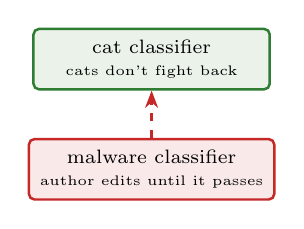
\begin{tikzpicture}[font=\scriptsize,node distance=6mm]
        \node[ok,minimum width=3.0cm] (cat) {cat classifier\\\tiny cats don't fight back};
        \node[hot,below=of cat,minimum width=3.0cm] (mal) {malware classifier\\\tiny author edits until it passes};
        \draw[attack] (mal.north) -- (cat.south);
      \end{tikzpicture}
    \end{column}
    \begin{column}{0.5\textwidth}
      \small Consequences we will unpack:
      \begin{itemize}\setlength\itemsep{1pt}
        \item the target moves \emph{on purpose} $\Rightarrow$ models decay;
        \item errors are not symmetric $\Rightarrow$ FP vs FN cost differs wildly;
        \item you must \emph{explain} a block, not just make it.
      \end{itemize}
    \end{column}
  \end{columns}
\end{frame}

\begin{frame}{The six hazards every security ML system faces}
  \footnotesize
  \begin{columns}[T]
    \begin{column}{0.5\textwidth}
      \begin{enumerate}\setlength\itemsep{3pt}
        \item \term{Adaptive adversary.} Attackers probe and adapt; a great model
              ages the moment it ships.
        \item \term{Data / concept drift.} ``Normal'' and ``malicious'' both
              change --- retrain or rot.
        \item \term{Class imbalance \& base rate.} 1 attack in a million events:
              even 99.9\% accuracy drowns you in false positives.
      \end{enumerate}
    \end{column}
    \begin{column}{0.5\textwidth}
      \begin{enumerate}\setlength\itemsep{3pt}\setcounter{enumi}{3}
        \item \term{False positives / negatives.} A FP wastes analysts; a FN is a
              breach. The threshold is a business decision.
        \item \term{Explainability.} ``The model said so'' will not survive an
              audit, a court, or an angry blocked user.
        \item \term{Adversarial ML.} Attacks \emph{on} the model itself
              --- next slide.
      \end{enumerate}
    \end{column}
  \end{columns}
  \vfill
    \begin{block}{Definitions}
    Recall: from all the malicious events, what fraction did we catch? It is defined as $\text{recall} = \frac{\text{TP}}{\text{TP + FN}}$.\\
    Precision: from all the events we flagged, what fraction were actually malicious? It is defined as $\text{precision} = \frac{\text{TP}}{\text{TP + FP}}$.\\
    False positive rate: from all the benign events, what fraction did we flag? It is defined as $\text{FPR} = \frac{\text{FP}}{\text{FP + TN}}$.
  \end{block}
  \myth{``99\% accuracy = great detector.'' With a 1-in-a-million base rate,
  accuracy is meaningless --- ask about false-positive \emph{rate} and recall.}
  % Note: the base-rate fallacy is worth a 60-second whiteboard aside (see guide).


\end{frame}

\begin{frame}{Adversarial machine learning --- the model is now a target}
  % Note: this slide seeds the rest of the lecture series. Keep it vivid, brief.
  \begin{columns}[T]
    \begin{column}{0.5\textwidth}
      \begin{block}{\small Evasion (at inference time)}
        \small Perturb the input just enough to flip the decision:
        add benign strings to malware, tweak pixels in a CAPTCHA, pad a packet.
        The file still works --- the model now says ``benign''.
      \end{block}
      \begin{block}{\small Poisoning (at training time)}
        \small Feed the training pipeline bad data so the model learns the
        \emph{wrong} boundary --- e.g.\ teach a spam filter that the attacker's
        words are ``ham''.
      \end{block}
    \end{column}
    \begin{column}{0.5\textwidth}
      \centering
      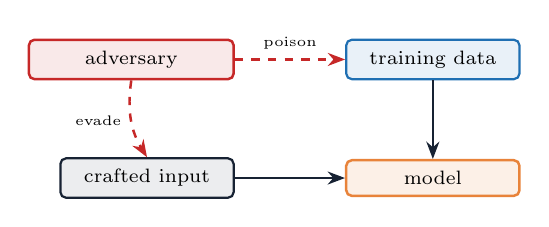
\begin{tikzpicture}[font=\scriptsize,node distance=6mm]
        \node[hot,minimum width=2.6cm] (adv) {adversary};
        \node[box,right=14mm of adv,minimum width=2.2cm] (train) {training data};
        \node[sig,below=10mm of train,minimum width=2.2cm] (model) {model};
        \node[darkbox,left=14mm of model,minimum width=2.2cm] (inp) {crafted input};
        \draw[attack] (adv) -- node[above,font=\tiny]{poison} (train);
        \draw[flow] (train) -- (model);
        \draw[attack] (adv.south) to[bend right=20] node[left,font=\tiny]{evade} (inp.north);
        \draw[flow] (inp) -- (model);
      \end{tikzpicture}
      \par\vspace{0.3em}
      {\footnotesize\color{midgray}Two entry points: corrupt what it \emph{learns},
      or fool what it \emph{sees}.}
    \end{column}
  \end{columns}
  \vfill
  {\footnotesize\color{midgray}These --- plus model theft, membership inference,
  and prompt injection --- are dedicated lectures later in this series.}
\end{frame}

%##############################################################################
%  PART IV -- PRACTICE & WRAP-UP
%##############################################################################

%==============================================================================
\section{The red thread}
%==============================================================================

\begin{frame}{The board: one picture of the whole lecture}
  % Note: reproduce this on the whiteboard as you go; reveal it complete here.
  \centering
  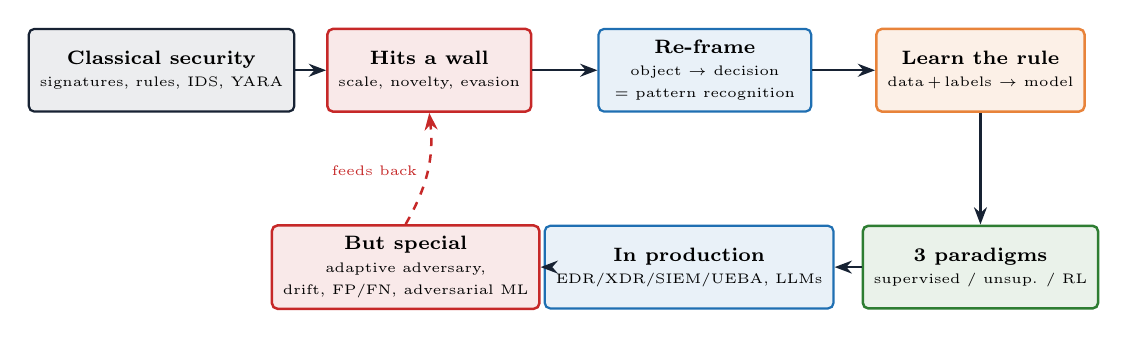
\begin{tikzpicture}[font=\scriptsize]
    % --- top row: left to right ---
    \node[darkbox,minimum width=2.6cm,minimum height=1.05cm] (a) at (0,0)
      {\textbf{Classical security}\\\tiny signatures, rules, IDS, YARA};
    \node[hot,minimum width=2.5cm,minimum height=1.05cm] (b) at (3.4,0)
      {\textbf{Hits a wall}\\\tiny scale, novelty, evasion};
    \node[box,minimum width=2.7cm,minimum height=1.05cm] (c) at (6.9,0)
      {\textbf{Re-frame}\\\tiny object $\to$ decision\\\tiny = pattern recognition};
    \node[sig,minimum width=2.5cm,minimum height=1.05cm] (d) at (10.4,0)
      {\textbf{Learn the rule}\\\tiny data\,+\,labels $\to$ model};
    % --- bottom row: right to left (serpentine, so no arrow crosses a box) ---
    \node[ok,minimum width=2.7cm,minimum height=1.05cm] (e) at (10.4,-2.5)
      {\textbf{3 paradigms}\\\tiny supervised / unsup. / RL};
    \node[box,minimum width=2.9cm,minimum height=1.05cm] (f) at (6.7,-2.5)
      {\textbf{In production}\\\tiny EDR/XDR/SIEM/UEBA, LLMs};
    \node[hot,minimum width=2.7cm,minimum height=1.05cm] (g) at (3.1,-2.5)
      {\textbf{But special}\\\tiny adaptive adversary,\\\tiny drift, FP/FN, adversarial ML};
    % --- flow ---
    \draw[flow] (a) -- (b);
    \draw[flow] (b) -- (c);
    \draw[flow] (c) -- (d);
    \draw[flow] (d) -- (e);          % straight down the right edge
    \draw[flow] (e) -- (f);          % right to left
    \draw[flow] (f) -- (g);          % right to left
    % feedback: short, near-vertical, in the clear gap under "Hits a wall"
    \draw[attack] (g.north) to[bend right=18]
      node[left,font=\tiny,text=bad]{feeds back} (b.south);
  \end{tikzpicture}
  \vfill
  {\footnotesize\color{midgray}Follow the arrows (a snake): the problem forced the
  re-frame, the re-frame invited learning, and learning brought new problems ---
  which loop back and drive the rest of the series.}
\end{frame}

\begin{frame}{Summary}
  So, is everyhing solved with ML?
  \begin{itemize}
    \item Remember, the idea to introduce ML was the \emph{scale, novelty and evasion} limits of classical security.
    \item ML is more adaptive, but new problems arise: Data Poisoning, Evasion, Concept Drift, Explainability, Base Rate Fallacy
    \item What do we do then? We introduce new security mechanisms: adversarial training, certified robustness, secure datasets, explainability, uncertainty estimation
    \item So, a typical pattern in computer science: a shift of paradigm solves some problems, but introduces new ones. The cycle continues.
  \end{itemize}
  \begin{block}{A recurring pattern in Computer Science}
  Machine Learning did not end the security arms race. It moved it. We no longer fight over rules—we fight over models.
  \end{block}

\end{frame}

% \begin{frame}{Think--pair--share (pick one, 4 minutes)}
%   % Note: run ONE live depending on time; others are backup / homework. Full
%   % facilitation notes in instructor_guide.tex.
%   \small
%   \begin{enumerate}\setlength\itemsep{5pt}
%     \item \textbf{Rule vs.\ model.} Take \term{DNS tunnelling}. First: write the
%           \texttt{if\dots then} rule you would deploy. Then: list the
%           \emph{features} you'd hand a classifier. Which is more robust to an
%           adversary --- and why?
%     \item \textbf{Choose the paradigm.} You must detect \emph{insider} data
%           theft, but you have almost no labelled examples of insiders. Supervised,
%           unsupervised, or reinforcement? Justify in one sentence.
%     \item \textbf{Cost of errors.} For an \emph{airport} malware scanner vs.\ a
%           \emph{consumer} email spam filter, which is worse --- a false positive
%           or a false negative? Set the threshold accordingly.
%   \end{enumerate}
%   \vfill
%   {\footnotesize\color{midgray}\emph{Think} alone (1\,min) $\to$ \emph{pair}
%   (2\,min) $\to$ \emph{share} two answers with the room (1\,min).}
% \end{frame}

\begin{frame}{Self-test --- three quick questions}
  \footnotesize
  \textbf{Q1.} A \term{zero-day} attack evades signature-based detection mainly
  because:\\
  \quad A) it is encrypted \quad B) no signature for it exists yet \quad
  C) it is too small \quad D) firewalls are disabled

  \vspace{0.7em}
  \textbf{Q2.} You must detect \emph{unknown} attacks and have \emph{no}
  labelled attack data. Best fit:\\
  \quad A) supervised classification \quad B) unsupervised anomaly detection\\
  \quad C) writing more YARA rules \quad D) reinforcement learning

  \vspace{0.7em}
  \textbf{Q3.} With 1 attack per 1{,}000{,}000 events, why is ``99.9\% accuracy''
  a bad headline?\\
  \quad A) accuracy can't be measured \quad
  B) the base rate makes false positives dominate\\
  \quad C) 99.9\% is impossible \quad D) anomalies don't exist

  \vspace{0.6em}
  {\footnotesize\color{midgray}Answers on the next slide --- decide before you
  turn the page.}
\end{frame}

\begin{frame}{Self-test --- answer key}
  \small
  \begin{tabular}{ll}
    \toprule \textbf{Q} & \textbf{Answer}\\ \midrule
    Q1 & \textbf{B} --- a signature encodes the \emph{past}; a zero-day is new, so nothing matches.\\
    Q2 & \textbf{B} --- no labels $\Rightarrow$ model ``normal'' and flag deviations (anomaly detection).\\
    Q3 & \textbf{B} --- at a 1-in-a-million base rate, even 0.1\% error $=$ 1{,}000 false alarms per million.\\
    \bottomrule
  \end{tabular}
  \vfill
  \begin{block}{\small If Q3 stung}
    \small That is the \term{base-rate fallacy} --- the single most important trap
    in security ML, and why analysts drown in alerts. We return to it in the
    detection-engineering lecture.
  \end{block}
\end{frame}

\begin{frame}{Key takeaways}
  \small
  \begin{itemize}\setlength\itemsep{2pt}
    \item Classical security \term{did not fail} --- it hit \emph{scale, novelty
          and evasion} limits that hand-written rules structurally cannot cross.
    \item Most security tasks are really \mlterm{classification} or
          \mlterm{anomaly detection}: \emph{object $\to$ decision}.
    \item \mlterm{ML} $=$ \emph{learn} the decision rule from \term{data},
          \term{features} and \term{labels} instead of writing it by hand.
    \item Three paradigms, three jobs: \mlterm{supervised} (labelled detection),
          \mlterm{unsupervised} (find normal / anomalies), \mlterm{reinforcement}
          (learn to act).
    \item Security ML is unique because the \term{adversary adapts} --- bringing
          drift, brutal base rates, explainability needs and \term{adversarial ML}.
  \end{itemize}
  \vfill
  {\footnotesize\color{midgray}You can now answer the opening question:
  \emph{why did ML become necessary in security at all?}}
\end{frame}

% ---- The one message ---------------------------------------------------------
{\setbeamertemplate{footline}{}
\begin{frame}[plain,noframenumbering]
  \vfill\centering
  {\color{mlsig}\rule{0.3\paperwidth}{2.5pt}}\\[1.0em]
  {\usebeamerfont{title}\color{mlink}The one message}\\[0.8em]
  \begin{minipage}{0.82\textwidth}
    \centering\large\color{mlink}
    Machine learning does \textbf{not replace} classical security --- \\[0.3em]
    it \textbf{extends} it everywhere explicit rules are no longer enough.
  \end{minipage}\\[1.2em]
  {\footnotesize\color{midgray}Signatures for the known. Learning for the new,
  the vast, and the changing. Together.}
  \vfill
\end{frame}}

%==============================================================================
\section{References}
%==============================================================================

\begin{frame}{References \& further reading}
  \footnotesize
  \begin{itemize}\setlength\itemsep{2pt}
    \item Sommer \& Paxson --- \emph{Outside the Closed World: On Using Machine
          Learning for Network Intrusion Detection}. IEEE S\&P, 2010.
          (The classic ``why security ML is hard'' paper.)
    \item Chio \& Freeman --- \emph{Machine Learning \& Security}. O'Reilly, 2018.
    \item Goodfellow, Bengio \& Courville --- \emph{Deep Learning}. MIT Press, 2016
          (intuition chapters).
    \item Biggio \& Roli --- \emph{Wild Patterns: Ten Years After the Rise of
          Adversarial Machine Learning}. Pattern Recognition, 2018.
    \item NIST AI 100-2 --- \emph{Adversarial Machine Learning: Taxonomy and
          Terminology}. NIST, current edition.
    \item MITRE \emph{ATLAS} --- Adversarial Threat Landscape for AI Systems
          (\link{atlas.mitre.org}).
    \item OWASP \emph{Top 10 for LLM Applications} --- prompt injection \& friends.
    \item AV-TEST malware statistics (\link{av-test.org/en/statistics/malware}).
    \item Apruzzese et al.\ --- \emph{The Role of Machine Learning in
          Cybersecurity}. ACM DTRAP, 2023.
  \end{itemize}
\end{frame}

\begin{frame}[plain,noframenumbering]
  \vfill\centering
  {\color{mlsig}\rule{0.16\paperwidth}{2.2pt}}\\[0.8em]
  {\usebeamerfont{title}\color{mlink}Thank you}\\[0.4em]
  {\color{midgray}\small Questions, counter-examples, and ``but what about\ldots'' welcome.}\\[1.0em]
  {\footnotesize\color{midgray}Prof.\ Dr.-Ing.\ Sebastian Schlesinger {\color{mlsig}\textbullet}
   HWR Berlin {\color{mlsig}\textbullet} Introduction to ML for Security}
  \vfill
\end{frame}

\end{document}
